%!TEX program = xelatex
%!TEX builder = basic

\documentclass{article}
\usepackage{xeCJK}
  \setCJKmainfont[BoldFont=黑体, ItalicFont = 仿宋]{楷体}
  \setCJKmonofont{黑体}
  \setmainfont{Times New Roman}
  \setmonofont{Consolas}
\usepackage{xltxtra}
\usepackage{./glossaries-cn}
\usepackage{tikz}
\usepackage{indentfirst}
\hypersetup{
  colorlinks = true,
  pdfborder  = {0 0 0},
  linkcolor  = red,
  citecolor  = green,
  bookmarksopen,
  bookmarksnumbered
}
\linespread{1.5}
\setlength{\parindent}{2em}
\setlength{\parskip}{5pt}
\usepackage{geometry}
\geometry
{
  left   = 1in,
  right  = 1in,
  top    = 1in,
  bottom = 1in
}
\usepackage{listings}
\lstdefinestyle{latexcode}{
  basicstyle   = \ttfamily\scriptsize,%
  breaklines   = true,%
  language     = [LaTeX]{TeX},
  keywordstyle = \color{black},
  texcsstyle   = \color{black}, 
  commentstyle = \color{green!50!black},
  frame        = shadowbox,
  numbers      = left,
  numberstyle  = \tiny,
  rulesepcolor = \color{black!50},
  firstnumber  = last
}

\lstset{
  style        = latexcode,
  basicstyle   = \ttfamily,
}

\usepackage[many]{tcolorbox}
\tcbuselibrary{theorems}
\tcbset{
  enhanced jigsaw,
  breakable,
  before skip    = 10pt,
  left           = 2pt,
  right          = 2pt,
  separator sign = { },
  before upper   = {},
  fonttitle      = \bfseries
}

\newtcbtheorem[no counter]{command}{命令}
{
  colback  = green!5,
  colframe = green!35!black
}{cmd}



\usepackage{unicode-math}
  \setmathfont[version=lm]{Latin Modern Math}
  \setmathfont[range={\mathscr, \mathbfscr}]{XITS Math}
  \setmathfont[range=\mathbb]{TeX Gyre Termes Math}
  \mathversion{lm}

\newcommand{\oarg}[1]{\texttt{[#1]}}
\newcommand{\marg}[1]{\texttt{\{#1\}}}
\newcommand{\var}[1]{$\langle\text{\it #1}\rangle$}
\renewcommand{\figurename}{图}
\renewcommand{\contentsname}{目录}
\renewcommand{\lstlistingname}{代码}

\NewTerm[phrase]     {ME}         {glossaries-cn}                                {glossaries-cn}
\NewTerm             {HUST}       {Huazhong University of Science \& Technology} {华中科技大学}
\NewTerm[no acronym] {AC}         {School of Automation}                         {自动化学院}
\NewTerm[no fullname]{233}        {23333333333333333333}                         {大笑}
\NewTerm[no acronym] {PCK}        {Package}                                      {宏包}
\NewTerm[no acronym] {term}       {Term}                                         {术语}
\NewTerm[phrase]     {default}    {}                                             {普通术语}
\NewTerm[phrase]     {no acronym} {}                                             {无英文缩写术语}
\NewTerm[phrase]     {no fullname}{}                                             {无英文全称术语}
\NewTerm[phrase]     {phrase}     {}                                             {固定搭配}
\NewTerm[phrase]     {chinese}    {}                                             {中文含义}
\NewTerm[phrase]     {fullname}   {}                                             {英文全称}
\NewTerm[phrase]     {acronym}    {}                                             {英文缩写}
\NewTerm[phrase]     {RA}         {}                                             {我也不知道叫什么名字比较好,随便起个名字先用着,以后再改吧}
\NewTerm[phrase]     {symbol}     {}                                             {数学符号}
\NewTerm[phrase]     {printsymbol}{}                                             {出现在符号表中的数学符号}
\NewTerm[phrase]     {hidesymbol} {}                                             {不出现在符号表中的数学符号}
\NewTerm             {IT}         {Information Technology}                       {信息技术}
\NewTerm             {DT}         {Data Technology}                              {数据技术}
\NewTerm[no acronym] {DotA}       {Defence of the Ancient}                       {DotA}
\NewTerm[phrase]     {Test1}      {}                                             {离散时间傅里叶变换}
\NewTerm[phrase]     {Test2}      {}                                             {离散 & 时间 & 傅里叶 & 变换}

\NewTerm[no acronym] {FT}         {Fourier Transform}                            {傅里叶变换}
\NewTerm[phrase]     {AFT}        {}                                             {傅里叶逆变换}
\NewTerm             {DTFT}       {Discrete-Time Fourier Transform}              {离散时间傅里叶变换}
\NewTerm             {DFT}        {Discrete Fourier Transform}                   {离散傅里叶变换}
\NewTerm             {FFT}        {Fast Fourier Transformation}                  {快速傅里叶变换}

\NewSymbol           {ABC}        {\triangle ABC}                                {直角三角形}
\NewSymbol           {a}          {a}                                            {直角三角形 $\gls{ABC}$ 的直角边}
\NewSymbol           {b}          {b}                                            {直角三角形 $\gls{ABC}$ 的直角边}
\NewSymbol           {c}          {c}                                            {直角三角形 $\gls{ABC}$ 的斜边}
\NewSymbol           {f}          {f}                                            {原函数}
\NewSymbol           {ff}         {\hat{f}}                                      {原函数 $\glsintoc{f}$ 的傅里叶变换}
\NewSymbol           {e}          {\mathrm{e}}                                   {自然对数的底}
\NewSymbol           {i}          {\mathrm{i}}                                   {虚数}
\NewSymbol           {pi}         {\pi}                                          {圆周率}

\definecolor{termcolor}{rgb}{0, .3, 0}
\definecolor{symbolcolor}{rgb}{0, 0, 1}
\glssetup{
  term list title    = 缩略词表,
  symbol list title  = 符号表,
  list level         = section,
  term color         = termcolor,
  symbol color       = symbolcolor,
  list head distance = -3.7em
}

\begin{document}
\begin{center}
\Large \texttt{\glsintoc{ME}} \glsintoc{PCK}使用说明\\[5pt]
\large 作者:张琦\\
\href{mailto:qiqi@hust.edu.cn}{qiqi@hust.edu.cn}\\
\today
\end{center}
\subpdfbookmark{\contentsname}{toc}
\tableofcontents

\PrintTermList

\PrintSymbolList

\section{介绍}
中文的\glsintoc{term}与英文的\gls{term} 不同,是因为中文除了\gls{fullname}和\gls{acronym}之外,还需要\gls{chinese},这导致 \LaTeX{} 自带的 \texttt{glossaries} \gls{PCK} 和 \texttt{datagidx} \gls{PCK}需要很多配置才能使用在中文的学位论文中。\texttt{\gls{ME}} \glsintoc{PCK}基于 \texttt{datagidx} \gls{PCK},并在 \texttt{datagidx} \gls{PCK}的基础上结合中文论文的特点做了一些特殊的定制,方便中文论文的写作。

中文论文中有 4 种\gls{term}:
\begin{itemize}
  \item \textbf{\gls{default}},含有\gls{chinese}、\gls{fullname}和\gls{acronym}。\gls{default}要求首次出现的格式为:
  \[
    \text{\var{\gls{chinese}}(\var{\gls{fullname}}, \var{\gls{acronym}}),}
  \]
  非首次出现的格式为:
  \[
    \text{\var{\gls{acronym}}。}
  \]
  比如:我来自\gls{HUST},\gls{HUST} 位于湖北省武汉市洪山区。
  \item \textbf{\gls{no acronym}},含有\gls{chinese}和\gls{fullname}。\gls{no acronym}要求首次出现的格式为:
  \[
    \text{\var{\gls{chinese}}(\var{\gls{fullname}}),}
  \]
  非首次出现的格式为:
  \[
    \text{\var{\gls{chinese}}。}
  \]
  比如:我来自 \gls{HUST} 的\gls{AC},\gls{AC}是由原控制科学与工程系和原图像识别与人工智能研究所于 2013 年合并组建的学院。
  \item \textbf{\gls{no fullname}},含有\gls{chinese}和\gls{acronym}。\gls{no fullname}要求首次出现的格式为:
  \[
    \text{\var{\gls{chinese}}(\var{\gls{acronym}}),}
  \]
  非首次出现的格式为:
  \[
    \text{\var{\gls{acronym}}。}
  \]
  比如:\gls{233} 的出处来自猫扑,因为猫扑的第 233 个表情是大笑的表情,所以人们用 \gls{233} 表示大笑。
  \item \textbf{\gls{phrase}},只含有\gls{chinese}。\gls{phrase}不论是首次出现还是非首次出现,其格式均为:
  \[
    \text{\var{\gls{chinese}}。}
  \]
  \gls{phrase}表示固定的词语搭配,一般用于在行文过程中还没有确定的名词。比如我设计了一个算法,但是算法的名字还没想好,但是这并不影响文章写作,就叫它\gls{RA}好了,行文过程中可以这样描述``\gls{RA}是一种贝叶斯网的近似推理方法''。
\end{itemize}
以上 4 种\gls{term}只有\gls{default}会出现在\gls{term}表中,其余 3 种\gls{term}因为缺少\gls{fullname}或者\gls{acronym}而不会出现在\gls{term}表中。

中文论文中有 2 种\gls{symbol}:
\begin{itemize}
  \item \textbf{\gls{printsymbol}},含有\gls{chinese}以及相应的 \LaTeX{} 代码。\gls{printsymbol}不论是首次出现还是非首次出现,其格式均为:
  \[
    \text{\var{\gls{symbol}}。}
  \]
  \gls{printsymbol}会出现在\gls{symbol}表中,比如 $\gls{a}, \gls{b}, \gls{c}$ 是直角三角形 $\gls{ABC}$ 三条边,其中 $\gls{a}, \gls{b}$ 是斜边,$\gls{c}$ 是直角边,如图 \ref{fig:Right Triangle} 所示。
  \begin{figure}[!htb]
    \centering
    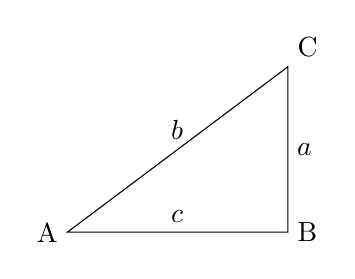
\begin{tikzpicture}[x = 0.7cm, 
                        y = 0.7cm]
      \coordinate (A) at (0, 0);
      \coordinate (B) at (4, 0);
      \coordinate (C) at (4, 3);
      \draw (A)                                   -- 
            (B)   node[midway, above] {$\gls{c}$} -- 
            (C)   node[midway, right] {$\gls{a}$} -- 
            cycle node[midway, above] {$\gls{b}$};
      \node[anchor = east]       at (A) {A}; 
      \node[anchor = west]       at (B) {B}; 
      \node[anchor = south west] at (C) {C}; 
    \end{tikzpicture}\vspace{-15pt}
    \caption{直角三角形 $\glsintoc{ABC}$}
    \label{fig:Right Triangle}
  \end{figure}
  \item \textbf{\gls{hidesymbol}},除了不会出现在\gls{symbol}表中,其它行为与\gls{printsymbol}基本一致。
\end{itemize}

\section{简明教程}
\subsection{新建\glsintoc{term}}
新建\gls{term}用 \lstinline{\NewTerm} 命令,其语法如下所示。
\begin{command}{\lstinline{\\NewTerm}}{}
\verb"\NewTerm"\oarg{\var{\gls{term}类型}}\marg{\var{标签}}\marg{\var{\gls{fullname}}}\marg{\var{\gls{chinese}}}
\end{command}
其中:
\begin{itemize}
  \item \var{\gls{term}类型}是可选参数,表示\gls{term}的类型,可选值如下所示:
  \begin{itemize}
    \item \lstinline{default},表示该\gls{term}是\gls{default},是\var{\gls{term}类型}的默认值;
    \item \lstinline{no acronym},表示该\gls{term}是\gls{no acronym};
    \item \lstinline{no fullname},表示该\gls{term}是\gls{no fullname};
    \item \lstinline{phrase},表示该\gls{term}是\gls{phrase}。
  \end{itemize}
  \item \var{标签}是必选参数,表示\gls{term}的\gls{acronym},也用于\gls{term}的引用。
  \item \var{\gls{fullname}}是必选参数,表示\gls{term}的\gls{fullname},可以留空。
  \item \var{\gls{chinese}}是必选参数,表示\gls{term}的\gls{chinese}。
\end{itemize}

\begin{lstlisting}[style   = latexcode,
                   caption = {\texttt{\backslash NewTerm} 命令举例},
                   label   = {lst:Example of NewTerm}]
%       术语类型      标签      英文全称                 中文含义
\NewTerm              {IT}      {Information Technology} {信息技术}
\NewTerm[no acronym]  {AC}      {School of Automation}   {自动化学院}
\NewTerm[no fullname] {233}     {}                       {大笑}
\NewTerm[phrase]      {default} {}                       {普通术语}
\end{lstlisting}

\subsection{新建\glsintoc{symbol}}
新建\gls{symbol}用 \lstinline{\NewSymbol} 命令,其语法如下所示。
\begin{command}{\lstinline{\\NewSymbol}}{}
\verb"\NewSymbol"\oarg{\var{\gls{symbol}类型}}\marg{\var{标签}}\marg{\var{{\rm \LaTeX{}} 代码}}\marg{\var{\gls{chinese}}}
\end{command}
其中:
\begin{itemize}
  \item \var{\gls{symbol}类型}是可选参数,表示\gls{symbol}的类型,可选值如下所示:
  \begin{itemize}
    \item \lstinline{default},表示该\gls{symbol}是\gls{printsymbol},是\var{\gls{symbol}类型}的默认值;
    \item \lstinline{hide},表示该\gls{symbol}是\gls{hidesymbol}。
  \end{itemize}
  \item \var{标签}是必选参数,用于\gls{symbol}的引用。
  \item \var{{\rm \LaTeX{}} 代码}是必选参数,\gls{symbol}的 \LaTeX{} 代码。
  \item \var{\gls{chinese}}是必选参数,表示\gls{symbol}的\gls{chinese}。
\end{itemize}

\begin{lstlisting}[style   = latexcode,
                   caption = {\texttt{\backslash NewSymbol} 命令举例},
                   label   = {lst:Example of NewSymbol}]
%         符号类型  标签  LaTeX 代码      中文含义
\NewSymbol          {ABC} {\triangle ABC} {直角三角形}
\NewSymbol          {a}   {a}             {直角三角形 $\gls{ABC}$ 的直角边}
\NewSymbol          {b}   {b}             {直角三角形 $\gls{ABC}$ 的直角边}
\NewSymbol[default] {c}   {c}             {直角三角形 $\gls{ABC}$ 的斜边}
\NewSymbol[hide]    {pi}  {\pi}           {圆周率}
\end{lstlisting}

\subsection{\glsintoc{term}及\glsintoc{symbol}的引用}
\texttt{\gls{ME}} \gls{PCK}提供了 2 个引用命令,分别是 \lstinline{\gls} 和 \lstinline{\glsintoc}。
\begin{command}{\lstinline{\\gls} 和 \lstinline{\\glsintoc}}{}
\verb"\gls"\marg{\var{标签}}\\
\verb"\glsintoc"\marg{\var{标签}}
\end{command}

\verb"\gls"\marg{\var{标签}}用于正文中的\gls{term}或者\gls{symbol}的引用。\texttt{\gls{ME}} \gls{PCK}会自动区分首次引用与非首次引用,并按照其类型对应的规则对 \lstinline{\gls} 命令进行展开。

\verb"\glsintoc"\marg{\var{标签}}用于标题中的\gls{term}或者\gls{symbol}的引用,其中标题包括 \lstinline{\chapter}、\lstinline{\section}、\lstinline{\subsection}、\lstinline{\caption} 等等命令。对于\gls{term},\lstinline{\glsintoc} 命令将展开为\gls{chinese};对于\gls{symbol},\lstinline{\glsintoc} 命令将展开为 \LaTeX{} 代码。\lstinline{\glsintoc} 命令不算首次引用,标题中的\gls{term}只会以\gls{chinese}的形式展开。

\subsection{\glsintoc{term}及\glsintoc{symbol}的打印}
\texttt{\gls{ME}} \gls{PCK}提供 2 个命令 \lstinline{\PrintTermList} 和 \lstinline{\PrintSymbolList} 分别用来打印\gls{term}表以及\gls{symbol}表。
\begin{command}{\lstinline{\\PrintTermList} 和 \lstinline{\\PrintSymbolList}}{}
\verb"\PrintTermList"\\
\verb"\PrintSymbolList"
\end{command}

命令 \lstinline{\PrintTermList} 和 \lstinline{\PrintSymbolList} 均无参数,使用方法是在需要打印\gls{term}表的地方插入 \lstinline{\PrintTermList},在需要打印\gls{symbol}表的地方插入 \lstinline{\PrintSymbolList} 即可。命令 \lstinline{\PrintTermList} 只打印\gls{default},按照\gls{acronym}的字母排序,而命令 \lstinline{\PrintSymbolList} 只打印\gls{printsymbol},按照定义的顺序培训。

\subsection{\glsintoc{PCK}设置}
\texttt{\gls{ME}} \gls{PCK} 提供了设置命令 \lstinline{\glssetup},用来设置 \texttt{\gls{ME}} \gls{PCK}的部分参数。
\begin{command}{\lstinline{\\glssetup}}{}
\verb"\glssetup"\marg{\var{配置命令}}
\end{command}

\begin{itemize}
  \item \var{配置命令}是必选参数,提供了 6 个配置选项:
  \begin{itemize}
    \item \texttt{term list title},用来设置\gls{term}表的标题,默认值是 \texttt{Term List}; 
    \item \texttt{symbol list title},用来设置\gls{symbol}表的标题,默认值是 \texttt{Symbol List};
    \item \texttt{list level},用来设置\gls{term}表和\gls{symbol}表的层级,默认值是 \texttt{section};
    \item \texttt{term color},用来设置\gls{term}被引用时的的颜色,默认值是 \texttt{black};
    \item \texttt{symbol color},用来设置\gls{symbol}被引用时的的颜色,默认值是 \texttt{black};
    \item \texttt{list head distance},用来设置\gls{term}表和\gls{symbol}表表头和第一行的间距,默认值是 \texttt{-2.7em}。
  \end{itemize}
\end{itemize}

本\gls{PCK}的使用说明中的配置如代码 \ref{lst:Example of glssetup} 所示。
\begin{lstlisting}[style   = latexcode,
                   caption = {\texttt{\backslash glssetup} 命令举例},
                   label   = {lst:Example of glssetup}]
\definecolor{termcolor}{rgb}{0, .3, 0}
\definecolor{symbolcolor}{rgb}{0, 0, 1}

\glssetup{
  term list title    = 缩略词表,      % 术语表的标题
  symbol list title  = 符号表,        % 数学符号表的标题
  list level         = section,       % 术语表和数学符号表的层级
  term color         = termcolor,     % 术语被引用的颜色
  symbol color       = symbolcolor,   % 数学符号被引用的颜色
  list head distance = -3.7em         % 术语表和数学符号表表头和第一行的间距
}
\end{lstlisting}

\section{高级设置}
\subsection{中文断词}
对于某些\gls{phrase},比如``\gls{Test1}'',如果采用代码 \ref{lst:New Phrase without Tokenization} 声明的话,该\gls{phrase}在引用的时候可以在任何地方换行,在某些行宽较短的场合会产生阅读不适,比如 \texttt{tikz} \gls{PCK}中的 \texttt{node} 节点。
\begin{lstlisting}[style   = latexcode,
                   caption = {无断词设置的\glsintoc{phrase}声明},
                   label   = {lst:New Phrase without Tokenization}]
\NewTerm[phrase] {Test1} {} {离散时间傅里叶变换}
\end{lstlisting}

如图 \ref{fig:Phrase without Tokenization} 所示,\gls{phrase}``\gls{Test1}''被放在了一个限制宽度的 \texttt{node} 节点中,这就导致\gls{phrase}``\gls{Test1}''在不该断词的地方断开了。
\begin{figure}[!htb]
  \centering
  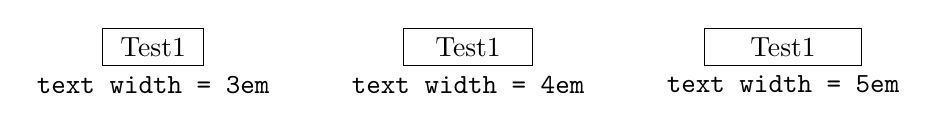
\begin{tikzpicture}[textbox/.style = {rectangle, draw, align = center, anchor = south},
                      node distance = 2.5cm]
    \linespread{1}
    \node[textbox, text width = 3em] (node1) at (0, 0) {\gls{Test1}};
    \node[textbox, text width = 4em] (node2) at (4, 0) {\gls{Test1}};
    \node[textbox, text width = 5em] (node3) at (8, 0) {\gls{Test1}};

    \node[anchor = north] at (node1.south) {\texttt{text width = 3em}};
    \node[anchor = north] at (node2.south) {\texttt{text width = 4em}};
    \node[anchor = north] at (node3.south) {\texttt{text width = 5em}};
  \end{tikzpicture}\vspace{-15pt}
  \caption{无断词设置的\glsintoc{phrase}引用}
  \label{fig:Phrase without Tokenization}
\end{figure}

为此,\texttt{\gls{ME}} \gls{PCK}提供了中文断词的设置,使用方法就是在 \lstinline{\NewTerm} 命令的 \var{\gls{chinese}} 参数中添加 \lstinline{&} 符号。\lstinline{&} 符号告诉 \LaTeX{} 系统只允许在 \lstinline{&} 处断词,其余位置禁止断词。\gls{phrase}``\gls{Test1}''正确的声明方法如代码 \ref{lst:New Phrase with Tokenization} 所示。

\begin{lstlisting}[style   = latexcode,
                   caption = {有断词设置的\glsintoc{phrase}声明},
                   label   = {lst:New Phrase with Tokenization}]
\NewTerm[phrase] {Test2} {} {离散 & 时间 & 傅里叶 & 变换}
\end{lstlisting}

用代码 \ref{lst:New Phrase with Tokenization} 声明的\gls{phrase}``\gls{Test2}''在 \lstinline{\gls} 命令中都会得到正确的断词,如图 \ref{fig:Phrase with Tokenization} 所示。

\begin{figure}[!htb]
  \centering
  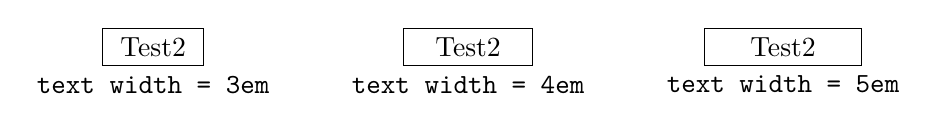
\begin{tikzpicture}[textbox/.style = {rectangle, draw, align = center, anchor = south},
                      node distance = 2.5cm]
    \linespread{1}
    \node[textbox, text width = 3em] (node1) at (0, 0) {\gls{Test2}};
    \node[textbox, text width = 4em] (node2) at (4, 0) {\gls{Test2}};
    \node[textbox, text width = 5em] (node3) at (8, 0) {\gls{Test2}};

    \node[anchor = north] at (node1.south) {\texttt{text width = 3em}};
    \node[anchor = north] at (node2.south) {\texttt{text width = 4em}};
    \node[anchor = north] at (node3.south) {\texttt{text width = 5em}};
  \end{tikzpicture}\vspace{-15pt}
  \caption{有断词设置的\glsintoc{phrase}引用}
  \label{fig:Phrase with Tokenization}
\end{figure}

建议利用 \texttt{\gls{ME}} \gls{PCK}声明\gls{term}的时候都使用断词设置。

\subsection{间距设置}
\XeLaTeX{} 在处理中文时会在全角字符和半角字符中间添加一定宽度的空白以保证美观。代码 \ref{lst:Example of Full and Half Characters} 中的三种写法编译后都是一样的效果,所以不需要人为的在全角字符和半角字符中间添加空格。

\begin{lstlisting}[style   = latexcode,
                   caption = {全角字符和半角字符混排},
                   label   = {lst:Example of Full and Half Characters}]
测试文字123测试文字abc测试文字
测试文字 123 测试文字 abc 测试文字
测试文字  123  测试文字  abc  测试文字
\end{lstlisting}

然而,\XeLaTeX{} 很难处理盒子与字符之间的空白,代码 \ref{lst:Example of Characters and Boxes} 中的两种写法编译后的效果是不同的,第 \ref{line:Wrong} 行渲染出来的效果是``测试文字\mbox{123}测试文字\mbox{abc}测试文字'',而第 \ref{line:Right} 行渲染出来的效果是``测试文字 \mbox{123} 测试文字 \mbox{abc} 测试文字''。显然,第 \ref{line:Right} 行是正确的写法。
\begin{lstlisting}[style      = latexcode,
                   caption    = {字符与盒子混排},
                   label      = {lst:Example of Characters and Boxes},
                   escapechar = |]
测试文字\mbox{123}测试文字\mbox{abc}测试文字 |\label{line:Wrong}|     % 错误的写法
测试文字 \mbox{123} 测试文字 \mbox{abc} 测试文字 |\label{line:Right}| % 正确的写法
\end{lstlisting}

\texttt{\gls{ME}} \gls{PCK}提供的 \lstinline{\gls} 命令和 \lstinline{\glsintoc} 命令本质上都是一个盒子,\XeLaTeX{} 无法正确处理 \lstinline{\gls} 命令和 \lstinline{\glsintoc} 命令与前后文之间的空白,故需要手动控制。代码 \ref{lst:Example of White Space} 展示了如何正确使用 \lstinline{\gls} 命令,注意代码 \ref{lst:Example of White Space} 中 \lstinline{\gls} 命令前后的空格符``\textvisiblespace''。
\begin{lstlisting}[style      = latexcode,
                   caption    = {正确使用 \texttt{\backslash gls} 命令},
                   label      = {lst:Example of White Space},
                   showspaces = true]
\NewTerm{IT} {Information Technology} {信息技术}
\NewTerm{DT} {Data Technology}        {数据技术}

\gls{DT} 与\gls{IT} 相对应,由马云在世界互联网大会中演讲时正式提出:`` \gls{IT} 和 \gls{DT} 是有巨大的差异,\gls{DT} 的核心,也就是互联网这一世纪最了不起的东西,利他主义,相信别人要比你重要,相信别人比你聪明,相信别人比你能干,相信只有别人成功,你才能成功。\gls{IT} 时代到 \gls{DT} 时代,最小的标志是你的思想,如何帮助别人成功。''
\end{lstlisting}

\gls{DT} 与\gls{IT} 相对应,由马云在世界互联网大会中演讲时正式提出:`` \gls{IT} 和 \gls{DT} 是有巨大的差异,\gls{DT} 的核心,也就是互联网这一世纪最了不起的东西,利他主义,相信别人要比你重要,相信别人比你聪明,相信别人比你能干,相信只有别人成功,你才能成功。\gls{IT} 时代到 \gls{DT} 时代,最小的标志是你的思想,如何帮助别人成功。''

\subsection{超链接}
也许你已经注意了,不论 \lstinline{\gls} 命令产生的引用还是 \lstinline{\glsintoc} 命令产生的引用,PDF 文档中的\gls{term}和\gls{symbol}都是以超链接的形式存在的。对于\gls{default}和\gls{printsymbol}来说,因为它们俩有对应的\gls{term}表和\gls{symbol}表,所以\gls{default}和\gls{printsymbol}的超链接是链接到\gls{term}表和\gls{symbol}表中的对应行。而对于\gls{no acronym}、\gls{no fullname}、\gls{phrase}和\gls{hidesymbol}来说,它们的超链接是链接到首次被引用的位置,因为首次被引用的位置往往有相应的介绍。

如果你想在第 4 次引用的时候才给出某个词的解释,那么,前面 3 个的调用可以使用 \lstinline{\glsintoc} 命令,第 4 个以及之后的引用都用 \lstinline{\gls} 命令就可以了,如代码 \ref{lst:trick of gls and glsintoc} 所示。此时点击``DotA''会跳转到有解释的那个``DotA''。
\begin{lstlisting}[style      = latexcode,
                   caption    = {\texttt{\backslash gls} 与 \texttt{\backslash glsintoc} 的灵活使用},
                   label      = {lst:trick of gls and glsintoc}]
经常听室友们说 \glsintoc{DotA} 的 \glsintoc{DotA} 的,那么 \glsintoc{DotA} 到底是什么?\gls{DotA} 可以译作守护古树、守护遗迹、远古遗迹守卫, 是由暴雪公司出品即时战略游戏《魔兽争霸 3》的一款多人即时对战、自定义地图,可支持 10 个人同时连线游戏,是暴雪公司官方认可的魔兽争霸的 RPG 地图。
\end{lstlisting}

经常听室友们说 \glsintoc{DotA} 的 \glsintoc{DotA} 的,那么 \glsintoc{DotA} 到底是什么?\gls{DotA} 可以译作守护古树、守护遗迹、远古遗迹守卫, 是由暴雪公司出品即时战略游戏《魔兽争霸 3》的一款多人即时对战、自定义地图,可支持 10 个人同时连线游戏,是暴雪公司官方认可的魔兽争霸的 RPG 地图。

\subsection{颜色设置}
本\gls{PCK}使用说明的颜色设置如代码 \ref{lst:Example of glssetup} 所示,\lstinline{\glssetup} 不光可以用在导言区,实际上,它可以用在任何位置,而且只会影响其后样式。如果你不习惯有颜色的超链接,在这里可以用代码 \ref{lst:Turn off Colorful Term Symbol} 将其关闭。虽然没有颜色了,但是超链接还是存在的,是可以点击的。

\begin{lstlisting}[style   = latexcode,
                   caption = {关闭彩色\glsintoc{term}和\glsintoc{symbol}},
                   label   = {lst:Turn off Colorful Term Symbol}]
\glssetup{
  term color   = black,
  symbol color = black
}
\end{lstlisting}

\glssetup{
  term color   = black,
  symbol color = black
}

之后的本\gls{PCK}的使用说明不论是\gls{term}还是\gls{symbol}都是黑色的。

\section{应用举例}
\gls{FT} 是一种分析信号的方法,它可分析信号的成分,也可用这些成分合成信号。许多波形可作为信号的成分,比如正弦波、方波、锯齿波等,\gls{FT}用正弦波作为信号的成分。\gls{FT}分为\gls{DFT}、\gls{DTFT} 以及\gls{FFT}。

\gls{DFT} 是\gls{FT}在时域和频域上都呈离散的形式;\gls{DTFT} 是\gls{FT}的一种,是 \gls{DFT} 之后进行采样的离散行数;\gls{FFT} 是 \gls{DFT} 的快速算法,它是根据 \gls{DFT} 的奇、偶、虚、实等特性,对 \gls{DFT} 的算法进行改进获得的。

\gls{FT}如公式 \eqref{eqn:Fourier Transform} 所示,\gls{AFT}如公式 \eqref{eqn:Inverse Transform} 所示。

\begin{equation}\label{eqn:Fourier Transform}
  \gls{ff} = \int_{-\infty}^{+\infty}\gls{f}(x)\gls{e}^{-2\gls{pi}\gls{i}x\xi}{\rm d}x
\end{equation}

\begin{equation}\label{eqn:Inverse Transform}
  \gls{f} = \int_{-\infty}^{+\infty}\gls{ff}(\xi)\gls{e}^{2\gls{pi}\gls{i}\xi x} {\rm d}\xi
\end{equation}

\begin{lstlisting}[style   = latexcode,
                   caption = {应用举例的 \LaTeX{} 代码},
                   label   = {lst:LaTeX Code of Example}]
% \NewTerm 和 \NewSymbol 需要放在导言区 
\NewTerm[no acronym] {FT}   {Fourier Transform}               {傅里叶变换}
\NewTerm[phrase]     {AFT}  {}                                {傅里叶逆变换}
\NewTerm             {DTFT} {Discrete-Time Fourier Transform} {离散时间傅里叶变换}
\NewTerm             {DFT}  {Discrete Fourier Transform}      {离散傅里叶变换}
\NewTerm             {FFT}  {Fast Fourier Transformation}     {快速傅里叶变换}
\NewSymbol           {f}    {f}                               {原函数}
\NewSymbol           {ff}   {\hat{f}}                         {原函数 $\gls{f}$ 的傅里叶变换}
\NewSymbol           {e}    {\mathrm{e}}                      {自然对数的底}
\NewSymbol           {i}    {\mathrm{i}}                      {虚数}
\NewSymbol[hide]     {pi}   {\pi}                             {圆周率}

% \begin{document}
% ...
\gls{FT} 是一种分析信号的方法,它可分析信号的成分,也可用这些成分合成信号。许多波形可作为信号的成分,比如正弦波、方波、锯齿波等,\gls{FT}用正弦波作为信号的成分。\gls{FT}分为\gls{DFT}、\gls{DTFT} 以及\gls{FFT}。

\gls{DTFT} 是\gls{FT}在时域和频域上都呈离散的形式,\gls{DTFT} 是\gls{FT}的一种。是 \gls{DFT} 之后进行采样的离散行数,\gls{FFT} 是 \gls{DFT} 的快速算法,它是根据 \gls{DFT} 的奇、偶、虚、实等特性,对 \gls{DFT} 的算法进行改进获得的。

\gls{FT}如公式 \eqref{eqn:Fourier Transform} 所示,\gls{AFT}如公式 \eqref{eqn:Inverse Transform} 所示。

\begin{equation}\label{eqn:Fourier Transform}
  \gls{ff} = \int_{-\infty}^{+\infty}\gls{f}(x)\gls{e}^{-2\gls{pi}\gls{i}x\xi}{\rm d}x
\end{equation}

\begin{equation}\label{eqn:Inverse Transform}
  \gls{f} = \int_{-\infty}^{+\infty}\gls{ff}(\xi)\gls{e}^{2\gls{pi}\gls{i}\xi x} {\rm d}\xi
\end{equation}
% ...
% \end{document}
\end{lstlisting}

\end{document}